\documentclass[conference]{IEEEtran}
\usepackage[pdftex]{graphicx}
\usepackage[cmex10]{amsmath}
\interdisplaylinepenalty=2500
\usepackage{array}
\usepackage{mdwmath}
\usepackage{mdwtab}
\usepackage{eqparbox}
\usepackage[font=footnotesize]{subfig}
\usepackage{fixltx2e}
\usepackage{url}
\hyphenation{}

% additional packages and utility commands

\usepackage{float}

\newcommand{\TODO}{\textbf{\color{red}TODO}}

% \usepackage{flushend}

% while preparing, linenumbers come in handy
\usepackage{lineno}
\setlength\linenumbersep{1mm}
\linenumbers

% until we settle on the final name ;-)
\usepackage{xspace}
\newcommand{\NAME}{id-foo\xspace}

% http://tex.stackexchange.com/questions/299/how-to-get-long-texttt-sections-to-break
\newcommand*\justify{%
  \fontdimen2\font=0.4em% interword space
  \fontdimen3\font=0.2em% interword stretch
  \fontdimen4\font=0.1em% interword shrink
  \fontdimen7\font=0.1em% extra space
  \hyphenchar\font=`\-% allowing hyphenation
}

% http://en.wikibooks.org/wiki/LaTeX/Customizing_LaTeX
\newcommand{\ttt}[1]{\texttt{\justify{#1}}}

\usepackage{algpseudocode}
% custom Let command
\newcommand*\Let[2]{\State #1 $\gets$ #2}
\renewcommand{\algorithmicforall}{\textbf{for each}}
\let\ForEach\ForAll

\usepackage{listings}

\usepackage{tikz}
\usetikzlibrary{positioning}
\usetikzlibrary{calc}
\usetikzlibrary{graphs}
\usetikzlibrary{trees}
\usetikzlibrary{arrows}

%!TEX root=paper.tex

% basics

\tikzset{
  box/.style            = { rectangle, minimum width=2cm, minimum height=1cm },
  border/.style         = { thick, draw=black },
  round/.style          = { rounded corners=3mm },
}

% system

\tikzset{
  artifact/.style       = { box, font=\ttfamily },
  support/.style        = { box, font=\itshape },
  user/.style           = { artifact, fill=black!15!white },
  dom/.style            = { support,  fill=black!30!white },
  platform/.style       = { support,  fill=black!55!white, text=white },
  native/.style         = { support,  fill=black!70!white, text=white },
  generated/.style      = { artifact, border, dashed },
  resource/.style       = { artifact, border },
  representation/.style = { support, border, round }
}

% UML

\tikzset{
  class/.style={
    box,
    border,
    text centered,
    text width=1.75cm
  },
  relation/.style       = { thick, draw=black, <-},
  subclass/.style       = { relation, >=open triangle 60 },
  aggregate/.style      = { relation, >=open diamond },
  composite/.style      = { relation, >=diamond },
  dependency/.style     = { relation, >=latex, -> }
}


\begin{document}

% to avoid syntax error highlighting - e.g. foo's not js ;-)
\expandafter\def\csname PY@tok@err\endcsname{}

\title{
\NAME: A framework for \\
Efficient Intrusion Detection\\
in the Internet of Things
}

\author{\IEEEauthorblockN{Christophe Van Ginneken, Jef Maerien, Christophe
Huygens, Danny Hughes, Wouter Joosen}%
\IEEEauthorblockA{iMinds-DistriNet, KU Leuven\\
3001 Leuven, Belgium\\
\{firstname.lastname\}@cs.kuleuven.be}}

\maketitle

\begin{abstract}

Supporting multiple intrusion detection (ID) algorithms imposes significant
overhead on Internet of Things (IoT) devices. Fusion of the underlying
algorithms can alleviate this, yet, proves to be time-consuming, repetitive and
error-prone. To address this problem we introduce \NAME, a framework for the
development of efficient intrusion detection systems (IDS). It consists of a
domain specific language (DSL) that allows formally describing ID algorithms on
a functional level. A code generator then fuses these algorithms and produces
more optimally organized source code. This way, \NAME addresses the
heterogeneity of both the IoT and ID, as well as the limited resources of IoT
devices. A side-by-side comparison shows that generated code reduces memory
footprint, message passing overhead and execution time in comparison to a
straightforward sequential implementation of the same algorithms.

\end{abstract}

\section{Introduction}

% context

% IoT + threat

The IoT presents a great potential to positively influence our daily work and
life: domotics, assisted living, e-health and enhanced learning are only a few
examples\cite{atzori2010internet}. But with this potential the IoT also
presents a significant threat: by opening our smart homes
\cite{aldrich2003smart} and personal data\cite{weber2010internet} to all these
interconnected devices, we also open them to everyone who is able to break the
virtual locks that protect them. IoT devices typically have limited batteries,
little processing power and memory is restricted to the bare minimum. These
properties make it hard to add any additional service, including security.

% classic networks: fw and central ids

In classic networks, firewalls focus on the outer perimeter of the network,
filtering unwanted packets and protecting the entire internal network. But
attacks on flaws in services can pass unnoticed. This is where intrusion
detection (ID) steps in: an ID probe monitors all traffic that passes through
the firewall, looking for patterns and optionally alerting the firewall if a
malicious pattern is detected\cite{denning1987intrusion}.

% manet: local ids -> localize -> limited resources

In wireless networks of resource constraint devices, which make up an
significant part of the IoT, it is not possible to have this single point in
the network that can oversee all traffic\cite{zhang2000intrusion,
mishra2004intrusion}. If the outer security perimeter diminishes, every device
has to implement its own lines of defense. But making the IDS a local service
on each device requires local resources, which are the scarce commodity to IoT
devices.

% gap analysis

Current developments in ID focus on programming frameworks to structure the
implementation of algorithms\cite{valero2012di} and offer the required basic
functional components to implement them\cite{krontiris2008lidea}. But they
don't offer a way to optimize the usage of resources. Nor do they support
systematic reuse to create different configurations for different devices.

% problem -> requirements for solution

The IoT is a heterogeneous environment, both in hardware and software.
Addressing this in a transparent and automated way is a key success factor for
any kind of development in this area. A solution that supports the integration
of multiple algorithms on IoT devices needs to consider the impact on their
resources. Different algorithms should be merged somehow to avoid accumulating
their impact.

% my approach merged into ...
% scientific contribution

% 1. framework: language + code generator

The first contribution of this paper is a framework that enables the formal
description of ID algorithms on a functional level. An automated code
generation process produces corresponding source code, for a given platform and
configuration. This way, the framework addresses the heterogeneous nature of
both the IoT and ID algorithms.

% 2. FCF to optimise

The second contribution introduces functional code fusion (FCF) as a generation
paradigm to solve the problem of hard to reuse and combine ID algorithms. FCF
identifies common data and functions, and organizes code in such a way that
redundant iterations, tests and computations are eliminated. Our results show
substantially improved memory usage, execution time and usage of the wireless
radio, reducing energy consumption.

% structure

The remainder of this paper proceeds as follows: section \ref{classification}
takes a look at ID algorithms and classifies them. Section \ref{pattern} looks
for patterns in the implementation of these classes of algorithms, details some
of the ideas behind FCF and identifies the different aspects of the problem
space. Section \ref{design} describes the design we applied to construct the
framework, its domain specific language (DSL) and code generator. Section
\ref{evaluation} evaluates an implementation and application of the framework.
Section \ref{related} explores related work in the field of DSLs for ID and
code generation for the IoT. Finally, section \ref{conclusion} summarizes our
findings, draws conclusions and identifies topics for future work.

\section{A Classification of ID Algorithms}
\label{classification}

Research into ID in wireless networks typically focuses on two major topics
that complement the architecture: the devices as single entities and the
network as a group of such devices. Both are important because the group cannot
make a decision without members that detect malicious behavior and a
group-based decision is often needed because nodes can easily miss out on
certain events that could indicate intrusions, due to their wireless and
not-always-on nature.

These two topics lead to the first two classes: detecting intrusions and
cooperative decision making. We also identify software attestation as a third
class. Although it can be considered as a special case of a combination of both
other classes, its focus is not on the detection of intrusions, but on the
effect of an intrusion on the system itself.

\subsection{Detecting Intrusions}
\label{detection}

There are different ways to construct a taxonomy for intrusion detection, but
common themes do appear. According to \cite{mishra2004intrusion} and
\cite{ioannis2007towards} there are three major categories: anomaly detection,
signature or misuse detection, and specification-based detection. In
\cite{alrajeh2013intrusion} the authors mostly agree with this topology, but
add the notion of hybrid intrusion detection systems and cross layer intrusion
detection systems as recent advances in research. Although these additional
categories offer very interesting prospects, the authors have to admit that the
impact on the resource-constrained devices might still be too much. We
therefore focus on the three categories agreed upon by most sources.

\begin{LaTeXdescription}
  
  \item[Anomaly detection] considers a baseline profile and evaluates all
  activity according to this profile. Aberrant behavior is flagged as a
  possible intrusion, but this is no exact science. The baseline profile can
  evolve over time, especially in wireless and mobile environments. The flagged
  incidents should therefore also be handled with care and no absolute
  decisions can be made from single events.
  
  \item[Signature or misuse detection] starts with known patterns of attacks
  and tries to find evidence in the actions of and communication with a device.
  Because many attacks use valid ways to communicate with services on the
  devices, this can also produce false positives and offers no black and white
  certainty.
  
  \item[Specification-based detection] uses constraints that describe the
  correct behavior of the system. Although that this approach can detect
  previously unknown attacks, it can sometimes not detect specific attacks that
  can be detected by anomaly or misuse detection.
  
\end{LaTeXdescription}

\subsection{Cooperative Decision Making}
\label{coorperative}

These taxonomies focus on the act of detecting intrusions themselves. In a
highly distributed environment, an orthogonal categorization, dealing with the
distributed nature of the network and its ways of communicating, may be even
more important.

As in many other situations, a group is often stronger than the sum of its
individual components. Because not all devices are always actively
participating in the network, some might miss clues that would otherwise lead
them to detect intrusions. It is hardly impossible for a single device to
detect a complex attack by itself. Therefore a second important research topic
consists of cooperative algorithms to combine information from single
identities into a group-based decision about alleged
intrusions\cite{zhang2000intrusion}. We identify two ways by which this
cooperative decision making can be constructed and focus on the way
participants exchange information: broadcasting and interactive.

\begin{LaTeXdescription}

  \item[Broadcasting] can sometimes allow a distributed, cooperative algorithm
  to be implemented locally. This is illustrated by the reputation-based
  detection algorithm introduced in \cite{ganeriwal2008reputation}, based on
  the same principle of a watchdog also found in \cite{mishra2004intrusion}
  Using this algorithm, nodes can exchange information about the reputation of
  other nodes, using only broadcasted messages. Combining this information
  allows them to decide about their trust in a given node, based on more than
  their own, often partial, observations alone.

  \item[Interactive] communication allows algorithms to exchange information to
  reach a consensus. In \cite{krontiris2009cooperative}, the authors first
  present a theoretical foundation to analyze cooperative algorithms. Given
  these foundations they continue to present an algorithm consisting of 5
  phases. It essentially implements a voting system-based on the Guy Fawkes
  protocol\cite{anderson1998new} to identify an intruder. It enables the
  exchange of suspected intruder information and allows distributed
  authentication of those \emph{votes}. Based on these authenticated votes, a
  distributed decision can be made about the commonly identified intruder.

\end{LaTeXdescription}

\subsection{Software Attestation}
\label{subsection:attestation}

A research topic that exists in parallel to the detection and cooperation
duality is software attestation. It offers algorithms for exchanging
information about the software that is running on a device, and aims to
identify devices that can no longer prove that their content is unaltered. A
family of algorithms to implement this functionality are
SWATT\cite{seshadri2004swatt}, ICE/SCUBA\cite{seshadri2006scuba} and
SAKE\cite{seshadri2008sake}.

Software attestation is hard and many details can cause an algorithm to fail. A
discussion surrounding this topic, started by \cite{castelluccia2009difficulty}
in response to the previously mentioned papers, illustrates this. In
\cite{perrig2010refutation} the authors of the original papers counter many of
the objections made to their work, but the general feeling is that even in the
best conditions, there is always a way to circumvent the most ingenious
algorithm to perform software-based attestation.

Within the context of this paper, we will not consider software attestation as
a special class and exclude it from our scope, only focusing on detecting
intrusions and distributed decision making.

Figure \ref{fig:classification} gives a visual overview of the classification
presented above.

\begin{figure}[!ht]
  \centering
  \scalebox{.85}{
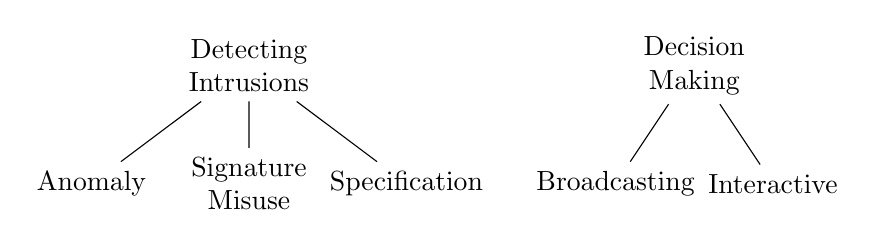
\begin{tikzpicture}[
  sibling distance=20mm,node distance=40mm
  ]
  \node (detection)             [align=center] {Detecting\\Intrusions}
    child {node (anomaly)       [align=center] {Anomaly}}
    child {node (signature)     [align=center] {Signature\\Misuse}}
    child {node (specification) [align=center] {Specification}};
  \node (decision)              [align=center,right=of detection] {Decision\\Making}
    child {node (broadcasting)  [align=center] {Broadcasting}}
    child {node (interactive)   [align=center] {Interactive}};
\end{tikzpicture}
}
  \caption{Classification of ID Algorithms}
  \label{fig:classification}
\end{figure}

\section{A Design Pattern for ID Algorithms}
\label{pattern}

Given this classification, we now introduce a design pattern that identifies
common aspects of these algorithms. It will allow us to define a strategy for
optimizing the combination of these algorithms. From the classification and
survey of several algorithms, we extract two activities common to most
algorithms: the inspection of network traffic and the evaluation of thresholds.

The former is trivial: network traffic is the carrier along which malicious
payloads reach the device or where patterns of communication can be observed
when other devices in the vicinity are affected by such payloads.

The latter is more complex: an algorithm based on signature or misuse detection
maybe sometimes can undeniably decide if an attack is real or not. But when
dealing with anomaly detection this line surely isn't that crisp. Especially in
distributed situations where even a neighboring device can not be trusted,
detecting intrusion is no absolute science. In this case one has to rely on
statistics and thresholds to decide when to drop trust in a given device.

Simply checking a threshold after updating some counter, is also not always a
good strategy. A simple example is that of a
watchdog\cite{mishra2004intrusion}, observing the actions of other devices.
There are valid reasons why a devices might miss the theoretical window in
which certain actions are expected. Simply reacting on such basic threshold
might result in false positives. A way to overcome this is to decouple the
detection of problems and the decision what to do about them.

This decoupling of detection and decision is the core of the design pattern for
ID algorithms. Listing \ref{alg:id-algo-pattern} presents the design pattern in
pseudo-code.

\begin{figure}[!ht]
\captionof{lstlisting}{ID Algorithm Pattern\label{alg:id-algo-pattern}}
\begin{algorithmic}[1]
  \Require{nodes, global storage for information about nodes}
  \Function{process\_message}{$msg$}
    \ForEach{$byte \in msg$} \label{alg:id-algo-pattern-loop1}
     \State \dots \Comment{analyze byte-sequences}
    \EndFor
    \Let{$nodes_x$}{value}  \Comment{optionally update node info}
    \State \Call{send}{$nodes_y$, ``info''} \Comment{optionally exchange info} \label{alg:id-algo-pattern-send1}
  \EndFunction
  \State
  \Function{do\_housekeeping}{}
    \ForEach{$node \in nodes$} \label{alg:id-algo-pattern-loop2} \label{alg:id-algo-pattern-common-data}
      \If{$node > \dots$} \Comment{validate recorded value}
        \State \dots \Comment{take actions}
        \State \Call{send}{$node$, ``info''} \Comment{e.g. communicate} \label{alg:id-algo-pattern-send2}
      \EndIf
    \EndFor
  \EndFunction
  \State
\end{algorithmic}
\end{figure}

We now extend the scope of the design pattern, to include its application in
the context of multiple algorithms. When implementing different algorithms, one
will typically encounter a pattern such as describes in listing
\ref{alg:id-algo-application}.

\begin{figure}[!ht]
\captionof{lstlisting}{Sequential implementation of ID algorithms\label{alg:id-algo-application}}
\begin{algorithmic}[1]
  \Let{$msg$}{$network$} \Comment{all observed messages}
  \ForEach{$algorithm \in algorithms$}
    \State \Call{algorithm.progress\_message}{msg}
  \EndFor
  \State \dots
  \Comment{at a given interval}
  \ForEach{$algorithm \in algorithms$}
    \State \Call{algorithm.do\_housekeeping}{}
  \EndFor
\end{algorithmic}
\end{figure}

The different implementations would be linked and called in a sequential way,
when new messages are observed on the network and at a regular interval to
allow them to do internal housekeeping, such as threshold evaluation. 

Given these patterns, we can now identify the problem areas that tend to result
in suboptimal code when combining multiple ID algorithms.

\subsection{Loops and Common Data}

Two issues arise from the nested loops that originate from the combination of
the ID algorithm patterns and its application pattern. First, each algorithm,
by itself, will parse each observed message on the network, processing the same
byte stream, performing comparable operation to find similar patterns.

Second, there is common data: Each algorithm also has to store information
about nodes within its own scope, resulting in a lot of duplicated information
in memory.

Reimplementing the algorithms manually to eliminate these issues is not a valid
option. This development cost typically isn't a one-time cost, e.g. in case a
new version of the algorithm is released, or simply when a different set of
algorithms is selected due to a changing risk analysis. Finally, changing, or
simply implementing the algorithms from scratch, also holds the risk of making
mistakes.

\subsection{Network Usage and Heterogeneity}

A third issue is hidden in the use of the network. The calls to the \ttt{SEND}
function are scattered around the algorithm, causing the wireless radio to be
accessed multiple times, keeping it active and energy consuming.

The heterogeneity of the IoT devices, results in many different software
stacks, each with their own network API. This also explains why there are very
few implementations readily available to developers: there is no common
platform to target for researchers.

Even using a unified software library would not only require a consistent
implementation of it, but would also limit the operational scope of the
research implementation, still restricting it to a single language.

\section{Design}
\label{design}

To bridge the gap between the research world and the heterogeneous IoT where
developers want to implement an actual IDS, while still respecting the limited
resources they have at their disposal, we introduce \NAME, a framework
consisting of a DSL, code generator and software library.

The DSL enables researchers to formally describe their ID algorithms, without
focusing on any specific language or platform. Given such formal descriptions
of ID algorithms, a code generator is now able to combine these, while avoiding
the problems arising from the patterns/problems presented in listings
\ref{alg:id-algo-application} and \ref{alg:id-algo-pattern}. It can also target
different languages and platforms, while reusing a software library that
provides e.g. message parsing, network access wrapping,\dots

\subsection{The Meaning of Loops}

From the design patterns we learned that loops are a major contributor to the
problem of algorithm fusibility. Loops in program code are technical constructs
and in fact often hide the actual intended functionality.

To illustrate this, we take the example of parsing network messages. Each
algorithm deals with parsing in the same way: loop over the bytes in the
payload and look for a pattern that identifies what the algorithm is looking
for. This is in fact a technical implementation choice. The underlying
functional goal is to react when such pattern is present in a message. The loop
has \emph{activated} this functionality, but the real goal is to
\emph{passively} react on an event, not \emph{actively} look for it.

This is how \NAME removes the need for loops: by introducing event handling,
constructions with loops are transformed to their functional meaning, allowing
much easier identification and fusion of common functionalities.

The same goes for actively polling some variable until it reaches a certain
threshold. This also can be transformed to an event, eliminating the need for a
technical loop-construction.

\subsection{A DSL for Nodes}

The second problem that could be observed from the patterns, was that of common
data. All algorithms deal with information about neighboring devices. To
centralize this information \NAME provides a unified \texttt{nodes} concept as
part of its DSL and exposes it as an object to the implementor.

Nodes can be extended with properties only available to the algorithm that
defines them. This way only one instance for every known devices will be
present in memory. Finally, nodes can define a scope for some function to be
executed in. This way, nodes also offer a way to iterate all known devices,
again without the need for a loop.

\subsection{Unified Messaging}

Sending and receiving of network messages is tightly integrated with the
previously mentioned concepts of event handling and the nodes domain. An
underlying software framework will handle all interaction with the network,
triggering functions by means of events when new messages are parsed and
exposing an API to send messages through the nodes domain. This approach gives
the framework complete control over the way messages are sent, allowing
optimized marshaling, grouping,\dots

Listing \ref{lst:watchdog} illustrates some of the features mentioned above,
using a small but representative example of an algorithm: a
watchdog\cite{mishra2004intrusion}. Like a heartbeat, nodes can broadcast a
message at a regular interval, allowing other nodes to monitor its
availability. Missing heartbeats could indicate problems, such as physical
capturing of a device.

\lstdefinelanguage{foo-lang}{
  emph={module,const,from,import,extend,with,after,do,function,@every,having},
  emphstyle={\textbf},
  morecomment=[l]{//},
  moredelim=[is][]{@@}{@@},       % temp solution to allow keywords without emph
  moredelim=[is][\emph]{!!}{!!}   % temp solution to hightlight #atoms
}

\lstinputlisting[
  language=foo-lang,
  float,
  basicstyle=\footnotesize\ttfamily\color{black},
  label=lst:watchdog,
  caption=Watchdog in \NAME
]{src/watchdog.foo}

\subsection{Code Generator}

To convert the DSL-based ID algorithms into production-ready code, we propose
the use of a code generator. Although many approaches here are applicable, like
template-based text expansion, XSLT transformations or even using the
CodeDom\cite{dollard2004code}, we believe that for the level of functional
transformations that need to be performed, a richer model is required.

A semantic model \cite{fowler2010domain}, tied closely to the DSL itself, can
fulfill this role. Semantic transformations can now be applied to create a
code-oriented model, comparable to the idea of CodeDom. From there on,
syntactic transformations an emit actual source code. Figure
\ref{fig:code-generation} shows the overall procedure.

\begin{figure}[ht]
  \centering
  \scalebox{.85}{
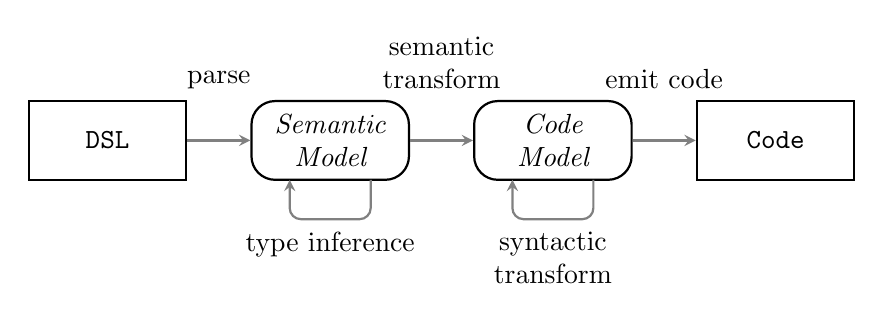
\begin{tikzpicture}[
  node distance=8mm,
  ,>=stealth,thick,black!50,text=black,
  every new ->/.style={shorten >=1pt}
]
  \node (dsl)  [resource]                                 {DSL};
  \node (sm)   [representation,right=of dsl,align=center] {Semantic\\Model};
  \node (cm)   [representation,right=of sm,align=center]  {Code\\Model};
  \node (code) [resource,right=of cm]        {Code};


  \draw [->] (dsl) -> (sm)   node [midway,above=15pt]              {parse};
  \draw [->] (sm)  -> (cm)   node [midway,above=15pt,align=center] {semantic\\transform};
  \draw [->] (cm)  -> (code) node [midway,above=15pt]              {emit code};

  \draw [rounded corners,->]
        ($ (sm.east) - (5mm,5mm) $)
        -- ++(0,-.5)
        -| ($ (sm.west) + (5mm,-5mm) $)
           node [near start, below=1pt] {type inference};

  \draw [rounded corners,->]
        ($ (cm.east) - (5mm,5mm) $)
        -- ++(0,-.5)
        -| ($ (cm.west) + (5mm,-5mm) $)
           node [near start, below=1pt,align=center] {syntactic\\transform};

\end{tikzpicture}
}
\caption{Overview code generation process}
\label{fig:code-generation}
\end{figure}

The DSL is parsed and imported into a semantic model. Based on the minimal type
information present in the model, all remaining types are inferred. Through a
series of semantic transformations, the model evolves from the functional to a
more technical one, a code model. This code model can be considered as a rich
abstract syntax tree (AST) with an extensive set of language constructs.
Syntactic transformations now lower this level of expressiveness according to
the desired platform and language. In the end the code model can be directly
emitted to the target language.

\subsection{Semantic Model}

The semantic model is the core of the solution. It offers a way to describe ID
algorithms in a way that allows semantic reinterpretation. This way, the
functionality of different algorithms can be reorganized to allow for more
optimal execution and memory usage. Hence the name \NAME of the framework:
intrusion detection functionality organization optimization.

Figure \ref{fig:meta-model} shows the central part of the semantic model as
implemented for \NAME.

\begin{figure}[ht]
  \centering
  \scalebox{.85}{
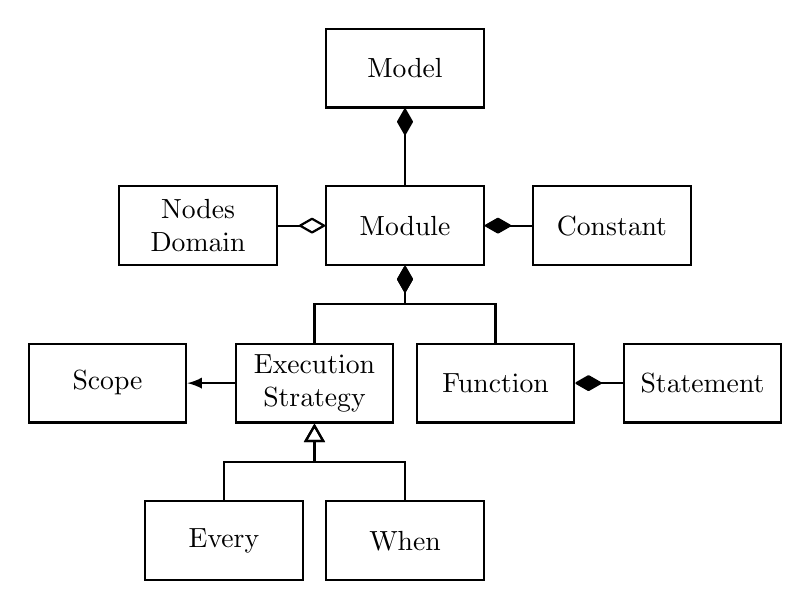
\begin{tikzpicture}[
  edge from parent fork down,
  sibling distance=5mm, level distance=20mm, node distance=6mm
  ]
  \node (model) [class] {Model}
      child {node (module) [class] {Module} edge from parent [composite]
        child {node (strategy) [class,align=center,xshift=-9mm] {Execution\\Strategy} edge from parent [composite]
          child {node(every) [class,xshift=-9mm] {Every} edge from parent [subclass]}
          child {node (when) [class,xshift=9mm] {When} edge from parent [subclass]}
        }
        child {node (function) [class,xshift=9mm] {Function} edge from parent [composite]}
      };
  \node (constant)  [class,right=of module]   {Constant};
  \node (scope)     [class,left=of strategy]  {Scope};
  \node (statement) [class,right=of function] {Statement};
  \node (nodes)     [class,left=of module]    {Nodes\\Domain};
  
  \draw [aggregate]  (module)   -- (nodes);
  \draw [composite]  (module)   -- (constant);
  \draw [dependency] (strategy) -- (scope);
  \draw [composite]  (function) -- (statement);
\end{tikzpicture}
}
\caption{Partial Semantic Model for \NAME}
\label{fig:meta-model}
\end{figure}

The concept driving this model is the structure starting at the \emph{Model} up
to the \emph{Execution Strategy}. This structure surrounds the actual
\emph{Function}s and underlying \emph{Statement}s and allows for interpretation
and fusion of the algorithms.

\subsection{Functional Code Fusion}

Thanks to the functional description of events and the effects that are
triggered by them, the code generator is able to identify the same actions
across different algorithms. This way it is possible to extract the parsing of
incoming messages, group actions on the same sets of data or scheduled function
executions.

FCF typically looks for patterns in the semantic model and performs model
transformations to change these patterns to a more optimized organization.
Semantic transformations are performed on the semantic model itself and end
with a transformation of the semantic model into a code model, which encodes
the semantics into technical code constructs.

\subsection{Code Model}

The code model can be compared to an AST for a very expressive language. It
contains constructs found in certain languages, but not in others. Therefore a
second round of model transformations needs to be performed. These syntactic
transformations morph the unsupported constructs into comparable constructs
that are supported by the targeted platform and language.

Depending on the target platform, some of the constructions used to e.g. parse
incoming messages, schedule tasks,\dots may not be transformed into
self-containing code. The generator then uses a software library to perform
these tasks. It will look for patterns that indicate any of these actions and
transform them into calls into the \NAME software library.

\subsection{Software Library}

We already touched upon the underlying software library when discussing the
unified messaging framework: incoming messages are parsed, outgoing messages
grouped. Besides these examples, other common functionality also isn't
generated. The execution of functions based on a schedule or the implementation
of higher level conceptual functions, such as \texttt{now} and \texttt{sha1},
are calls into the standard software library that supports the code generator.

\section{Implementation and Evaluation}
\label{evaluation}

To evaluate the prototype we chose to use a system based on the Atmel
ATMEGA1284p micro-controller \cite{datasheet:atmega1284p} and the Digi XBee S2
ZigBee module \cite{manual:xbee}. To drive the hardware a minimalistic library
was used, wrapping the technical calls to the components in more easy to use
functions.

The reason for this at first sight unusual setup is simple: relying on basic
hardware and software allows us to validate that the generator is capable of
generating code even for the most basic environment available. Any step up,
both in hardware or software, would offer better and higher abstractions that
would make it easier to generate code for that situation. It shows that the
requirements of the generator towards the platform are minimal, don't rely on
advanced frameworks or operating systems and can therefore be applied in any
environment, targeting any platform.

For the evaluation we constructed a small meshed network consisting of three
devices, with only one device able to talk to both other devices, requiring
routing of messages through this device.

We started from a basic application that measures light intensity. The
application was written both manually and generated. On top of this baseline we
added two intrusion detection related algorithms: a heartbeat, that allows
nodes to validate each other's continuous presence, and a reputation-building
algorithm that checks if a parent node is cooperative and actually forwards
messages with a destination further down the
network\cite{ganeriwal2008reputation}.

Three criteria were evaluated: the image size of the resulting compiled code,
the network usage in number of frames and bytes and the time required to
perform once cycle of the event loop. These metrics were collected in four
situations: without ID algorithms, with a heartbeat, with reputation-tracking
and with both algorithms implemented.

In case of the manual implementation, both algorithms were constructed as
standalone modules and sequentially called from the base-application's event
loop. The code generator was provided with \NAME descriptions of the algorithms
and generated all four cases.

Before reviewing the results, it is very important to put these results in a
proper perspective. Comparing manually written code to generated code is no
exact science. One can always argue that the quality of the two code bases is
not comparable and that the manual code always can be improved. Still it might
be interesting to look at the numbers, given that both code bases are
constructed with the same intentions and practices. We believe we have achieved
this and have taken honest decisions while constructing the implementations,
making them comparable. Numerical analysis of the implementation offers us a
preliminary estimation of the effect of our proposed solution.

Tables \ref{tbl:manual} and \ref{tbl:generated} show the collected data
respectively for the manual and the generated implementation. The base case is
presented in absolute values, while the implementations with the added
algorithms are presented as relative values.

\begin{table}[H]
  \centering
  \begin{tabular}{lrrrr}
  \hline
      & base & heartbeat & reputation & both\\
  \hline
  size (bytes) & 10500 & 148\% & 127\% & 175\%\\
  frames & 20 & 255\% & 160\% & 315\%\\
  bytes & 476 & 406\% & 181\% & 487\%\\
  time ($\mu$s) & 48 & 196\% & 183\% & 310\%\\
  \hline
  \end{tabular}
  \caption{Results for the manual implementation.}
  \label{tbl:manual}
\end{table}

\begin{table}[H]
  \centering
  \begin{tabular}{lrrrr}
  \hline
         & base & heartbeat & reputation & both\\
  \hline
  size (bytes) & 10496 & 175\% & 156\% & 200\%\\
  frames & 20 & 245\% & 160\% & 275\%\\
  bytes & 476 & 399\% & 186\% & 454\%\\
  time ($\mu$s) & 48 & 252\% & 252\% & 288\%\\
  \hline
  \end{tabular}
  \caption{Results for the generated implementation.}
  \label{tbl:generated}
\end{table}

From these raw results, we learn that adding algorithms manually to the
base-application, results in a cumulative increase. The impact of both
algorithms is simply the sum of the impact of each algorithm by itself. In the
case of the time required to execute one cycle of the event loop, the total
time is even a bit higher than simply the sum.

In the case of the generated implementation, this no longer holds: although
that even the individual increases due to adding a single algorithm are higher
than in the manual case, the result for the implementation of both algorithms
is less than the sum of both. Here we clearly see the effect of reusing the
software library that comes with \NAME. The same goes for all other metrics.
Maybe most remarkable is the effect on the time of one event loop cycle: both
algorithms by itself add 150\% with respect to the base case, but when
combined, the impact hardly increases. Here we learn that the introduced
software library is responsible for the initial overhead, but it clearly pays
for itself when adding more algorithms.

Table \ref{tbl:summary} compares the two situations by subtracting the manual
case from the generated case, showing the impact of the code generation. A
relative value for the entire implementation with both algorithms is also
presented.

\begin{table}[H]
  \centering
  \begin{tabular}{lrrrrr}
  \hline
                & base & heartbeat & reputation & both  & result \\
  \hline
  size (bytes)  & -4    & 2822     & 3070       & 2664  & 115\%  \\
  frames        & 0     & -2       & 0          & -8    & 87\%   \\
  bytes         & 0     & -36      & 24         & -156  & 93\%   \\
  time ($\mu$s) & 0     & 27       & 33         & -11   & 93\%   \\
  \hline
  \end{tabular}
  \caption{Comparison of both implementations.}
  \label{tbl:summary}
\end{table}

When comparing the results of both implementations we first can conclude that
the generator produces exactly the same code for the base case. We couldn't
measure any real differences between both implementations.

Secondly, we see that the software library that comes with the generated code
adds to the size of the resulting image. But the cost is almost constant and is
relatively lower when algorithms are combined. With roughly 3KB of additional
overhead, or 15\% in this simple case, this impact is affordable.

From a functional point of view, the generated code lives up to the
expectations: both the number of frames as the bytes sent benefit from well
organized code and reuse of a common software library.

Finally we see that both algorithms by itself add an equal amount of time to
the processing of a single event loop cycle, but when combined, the event loop
is about 7\% faster compared to the manual case.

Without any effort to optimize the software library, nor leveraging knowledge
about the specific algorithms, this very basic generated code shows that the
proposed principles are not only theoretically feasible but actually result in
interesting improvements.

\section{Related Work}
\label{related}

\TODO

IDS in WSN \cite{perrig2004security,mishra2004intrusion}

DSL \cite{fowler2010domain,mernik2005and}

DSL for WSN \cite{naumowicz2009prototyping,levis2004tinyscript}

DSL for IDS \cite{eckmann2002statl}

Code Generation for embedded systems/WSNs \cite{leupers2000code,marwedel2002code}

Code Optimization for embedded systems/WSNs \cite{panda2001data,naik2001software}

Code Generation for IDS \cite{charitakis2003code}

% manet: IDS algorithms -> coorporation, trust

More than in a classic network IDS, ID algorithms for MANETS operate with a
large degree of uncertainty. They often have to collaborate with other devices
in the network \cite{marchang2008collaborative,krontiris2009cooperative}, which
increases the level of uncertainty, because no other device can fully be
trusted. An IDS on an IoT device will be able to provide the services with
information about the reputation \cite{ganeriwal2008reputation} of other nodes
in the network.

\section{Conclusion and Future Work}
\label{conclusion}

theoretical gains are met in practice

explore more domains + implement corresponding DSLs for embedded systems

extract generic language as host for DSLs

Integration of applications with generated IDS allows actively and dynamically
responding to changes in the reputation of other nodes.

The services running on those devices can take advantage of these local
security layers. If the IDS detects a problem, the service can immediately
terminate the communication with the attacker, before it's actually abused.

\section*{Acknowledgements}

This research is partially funded by the Interuniversity Attraction Poles
Programme Belgian State, Belgian Science Policy, and by the Research Fund KU
Leuven. This research is partially funded by the EU FP7 project NESSoS. We
would like to thank the reviewers for their thoughtful and helpful comments
that enhanced the readability of this paper. Our gratitude and respect also
goes out to all members of the NES task force at KU Leuven/DistriNet for
creating the nurturing environment where these ideas could grow.

\bibliographystyle{IEEEtran}
\bibliography{literature/referenties}

\end{document}
